% Convert to svg using pdf2svg or https://pdftoimage.com/pdf-to-svg

\documentclass{standalone}
\usepackage{tikz}
\usetikzlibrary{positioning, arrows.meta}

\usepackage{bm}
\newcommand{\mat}[1]{{\mathbf{{#1}}}}
% \newcommand{\vect}[1]{{\mathbf{#1}}}
\newcommand{\vect}[1]{{\bm{#1}}}
\newcommand{\x}[0]{\vect{x}}
\newcommand{\y}[0]{\vect{y}}

\begin{document}
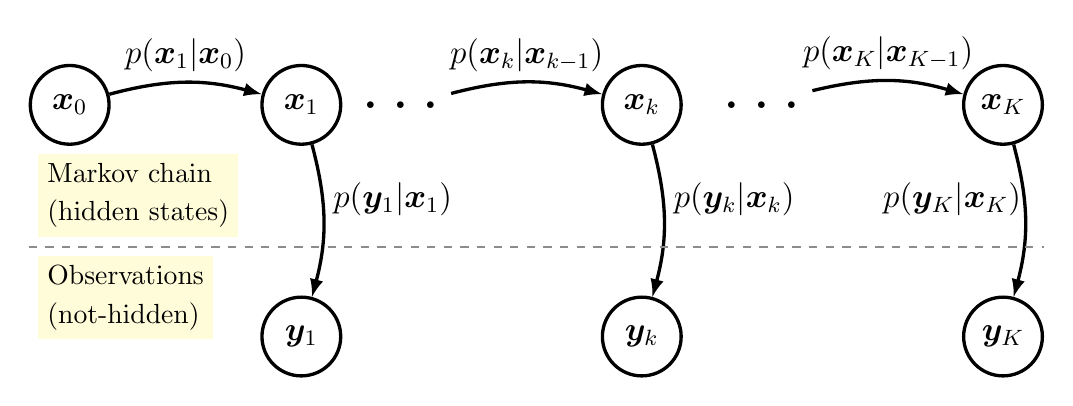
\begin{tikzpicture}[
    very thick,
    font=\large,
    state/.style={circle, draw, minimum size=1cm, text centered, inner sep=0pt},
    obs/.style={circle, draw, minimum size=1cm, text centered, inner sep=0pt},
    arrow/.style={-latex},
    node distance=1.9cm
]
% States
\node[state] (x0) {$\x_0$};
\node[state, right=of x0] (x1) {$\x_1$};
\node[right=3mm of x1] (x2dots) {\Huge \hspace{-2mm}$\dots$};
\node[state, right=of x2dots] (xk) {$\x_k$};
\node[right=3mm of xk] (xkdots) {\Huge \hspace{-2mm} $\dots$};
\node[state, right=of xkdots] (xK) {$\x_K$};

% Observations
% \node[obs, below=of x0] (y0) {$\y_0$};
\node[obs, below=of x1] (y1) {$\y_1$};
\node[obs, below=of xk] (yk) {$\y_k$};
\node[obs, below=of xK] (yK) {$\y_K$};

% Dynamical model
\draw[arrow] (x0) to[bend left=15] node[midway, above] {$p(\x_1 | \x_{0})$} (x1);
\draw[arrow] (x2dots) to[bend left=15] node[midway, above] {$p(\x_k | \x_{k-1})$} (xk);
\draw[arrow] (xkdots) to[bend left=15] node[midway, above] {$p(\x_K | \x_{K-1})$} (xK);

% Observation model
% \draw[arrow] (x0) to[bend left=15] node[pos=0.35, left] {$\mathcal{H}_0$} (y0);
\draw[arrow] (x1) to[bend left=15] node[pos=0.35, right] {$p(\y_1 | \x_1)$} (y1);
\draw[arrow] (xk) to[bend left=15] node[pos=0.35, right] {$p(\y_k | \x_k)$} (yk);
\draw[arrow] (xK) to[bend left=15] node[pos=0.35, left, xshift=1mm] {$p(\y_K | \x_K)$} (yK);

% Horizontal line and labels
\draw[dashed, draw=gray!90, line width=0.7pt] (x0.west |- 0,-1.8) -- (xK.east |- 0,-1.8);
\node[anchor=south west, align=left, fill=yellow!15, xshift=1mm] at (x0.west |- 0,-1.7) {\normalsize Markov chain\\\normalsize(hidden states)};
\node[anchor=north west, align=left, fill=yellow!15, xshift=1mm] at (x0.west |- 0,-1.9) {\normalsize Observations\\\normalsize(not-hidden)};


\end{tikzpicture}
\end{document}
